% This is "sig-alternate.tex" V2.0 May 2012
% This file should be compiled with V2.5 of "sig-alternate.cls" May 2012
%
% This example file demonstrates the use of the 'sig-alternate.cls'
% V2.5 LaTeX2e document class file. It is for those submitting
% articles to ACM Conference Proceedings WHO DO NOT WISH TO
% STRICTLY ADHERE TO THE SIGS (PUBS-BOARD-ENDORSED) STYLE.
% The 'sig-alternate.cls' file will produce a similar-looking,
% albeit, 'tighter' paper resulting in, invariably, fewer pages.
%
% ----------------------------------------------------------------------------------------------------------------
% This .tex file (and associated .cls V2.5) produces:
%       1) The Permission Statement
%       2) The Conference (location) Info information
%       3) The Copyright Line with ACM data
%       4) NO page numbers
%
% as against the acm_proc_article-sp.cls file which
% DOES NOT produce 1) thru' 3) above.
%
% Using 'sig-alternate.cls' you have control, however, from within
% the source .tex file, over both the CopyrightYear
% (defaulted to 200X) and the ACM Copyright Data
% (defaulted to X-XXXXX-XX-X/XX/XX).
% e.g.
% \CopyrightYear{2007} will cause 2007 to appear in the copyright line.
% \crdata{0-12345-67-8/90/12} will cause 0-12345-67-8/90/12 to appear in the copyright line.
%
% ---------------------------------------------------------------------------------------------------------------
% This .tex source is an example which *does* use
% the .bib file (from which the .bbl file % is produced).
% REMEMBER HOWEVER: After having produced the .bbl file,
% and prior to final submission, you *NEED* to 'insert'
% your .bbl file into your source .tex file so as to provide
% ONE 'self-contained' source file.
%
% ================= IF YOU HAVE QUESTIONS =======================
% Questions regarding the SIGS styles, SIGS policies and
% procedures, Conferences etc. should be sent to
% Adrienne Griscti (griscti@acm.org)
%
% Technical questions _only_ to
% Gerald Murray (murray@hq.acm.org)
% ===============================================================
%
% For tracking purposes - this is V2.0 - May 2012

\documentclass{sig-alternate}

\usepackage{url}

\begin{document}
%
% --- Author Metadata here ---
\conferenceinfo{Workshop on the theory and practice of social machines @ WWW2013}{2013, Rio de Janeiro, Brazil}
%\CopyrightYear{2007} % Allows default copyright year (20XX) to be over-ridden - IF NEED BE.
%\crdata{0-12345-67-8/90/01}  % Allows default copyright data (0-89791-88-6/97/05) to be over-ridden - IF NEED BE.
% --- End of Author Metadata ---

\title{``The Crowd Keeps Me in Shape'': Social Psychology and the Present and Future of Health Social Machines}
%
% You need the command \numberofauthors to handle the 'placement
% and alignment' of the authors beneath the title.
%
% For aesthetic reasons, we recommend 'three authors at a time'
% i.e. three 'name/affiliation blocks' be placed beneath the title.
%
% NOTE: You are NOT restricted in how many 'rows' of
% "name/affiliations" may appear. We just ask that you restrict
% the number of 'columns' to three.
%
% Because of the available 'opening page real-estate'
% we ask you to refrain from putting more than six authors
% (two rows with three columns) beneath the article title.
% More than six makes the first-page appear very cluttered indeed.
%
% Use the \alignauthor commands to handle the names
% and affiliations for an 'aesthetic maximum' of six authors.
% Add names, affiliations, addresses for
% the seventh etc. author(s) as the argument for the
% \additionalauthors command.
% These 'additional authors' will be output/set for you
% without further effort on your part as the last section in
% the body of your article BEFORE References or any Appendices.

\numberofauthors{1} %  in this sample file, there are a *total*
% of EIGHT authors. SIX appear on the 'first-page' (for formatting
% reasons) and the remaining two appear in the \additionalauthors section.
%
\author{
% You can go ahead and credit any number of authors here,
% e.g. one 'row of three' or two rows (consisting of one row of three
% and a second row of one, two or three).
%
% The command \alignauthor (no curly braces needed) should
% precede each author name, affiliation/snail-mail address and
% e-mail address. Additionally, tag each line of
% affiliation/address with \affaddr, and tag the
% e-mail address with \email.
%
% 1st. author
\alignauthor
Authors\\
       \affaddr{Web and Internet Science Group}\\
       \affaddr{University of Southampton}\\
       \affaddr{Southampton, UK}\\
       \email{\{a,b,c,d,e,f\}@ecs.soton.ac.uk}
}
% There's nothing stopping you putting the seventh, eighth, etc.
% author on the opening page (as the 'third row') but we ask,
% for aesthetic reasons that you place these 'additional authors'
% in the \additional authors block, viz.
%\additionalauthors{Additional authors: John Smith (The Th{\o}rv{\"a}ld Group,
%email: {\texttt{jsmith@affiliation.org}}) and Julius P.~Kumquat
%(The Kumquat Consortium, email: {\texttt{jpkumquat@consortium.net}}).}
%\date{30 July 1999}
% Just remember to make sure that the TOTAL number of authors
% is the number that will appear on the first page PLUS the
% number that will appear in the \additionalauthors section.

\maketitle
\begin{abstract}

Can the Web help people live healthier lives?  This paper seeks to
answer this question through an examination of sites, apps and online
communities designed to help people improve their fitness, better
manage their disease(s) and conditions, and to solve the often elusive
connections between the symptoms they experience, diseases and
treatments.  These \emph{health social machines} employ a combination
of both simple and complex social and computational processes to
provide such support.  We first provide a descriptive classification
of the kinds of machines currently available, and the support each
class offers.  We then describe the limitations exhibited by these
systems and potential ways around them, towards the design of more
effective machines in the future.

\end{abstract}

% A category with the (minimum) three required fields
%\category{H.4}{Information Systems Applications}{Miscellaneous}
%A category including the fourth, optional field follows...
%\category{D.2.8}{Software Engineering}{Metrics}[complexity measures, performance measures]

%\terms{Theory}

%\keywords{ACM proceedings, \LaTeX, text tagging}

\section{Introduction}

Health and well-being are visible indicators of technological
progress, as advances in healthcare and medicine are invariably
reflected in increases in average lifespan, reduction of disease and
suffering, and shortening of time needed to recover from illness and
injury.  As such, it is natural to ask how and whether the Internet
and the Web, two of the most significant inventions in recent human
history, have or may have an effect on health and wellbeing.

In this position paper, we examine a specific class of systems enabled
by the Web and pervasive Internet-enabled systems, which we call
\emph{health social machines}.  We define health social machines to
encompass a broad class of systems that provide
technologically-mediated interaction of large groups of individuals,
typically via a website, app, and sensor-based online community.
Individuals usually communicate and interact, directly or indirectly,
through some mediated or moderation mechanisms, in order to
collectively accomplish or address a health-related problem or need
\cite{hendler2010semantic}.  Such problems, as we illustrate through
examples we provide later, may be on the scale of an individual's
disease or well-being management, to that of contributing evidence and
insight to fundamental questions at the frontier of modern medicine.

We first describe the emerging landscape of health-related social
machines, identifying sets of classes and characteristics such
machines typically exhibit.  We then focus on specific challenges
faced by these classes in the longer term, and how emerging insights
from behavioural ecnonomics and technological platforms may address
some of these needs.

\section{Current Health Social Machines: A Brief Classificatory Analysis}

We first collected examples of popular health social machines through
a iterative process which started with filtering several popular blogs
focused on health-technology, the ``quantified-self'' and ``life
hacking'', for announcements related to apps and websites dedicated to
addressing health issues. We then clustered the collected candidates
using a Grounded Theory approach.  This process yielded three,
partially overlapping clusters of machines by the ways these machines
sought to address health needs.  Table \ref{table:clusters} these
clusters, comprising \emph{behavioural intervention}, \emph{disease
  management}, and \emph{collective sensemaking} of symptoms, and
associated machines falling in each category.

\subsection{Behavioural Intervention}

The first which we refer to as \emph{behavioural intervention
  machines} are systems that seek to help individuals achieve certain
health related-goals by altering their daily routine(s) and
activities.  The majority of systems we found in this category, which,
itself is the largest of the three categories, aim to help individuals
increase their general activity levels to increase fitness.  Since
these systems generally do not target any particular demographics or
those conditions, we consider them general, preventative health
machines with a focus on increasing fitness.

A large number, but not all, of such fitness machines either require,
or are designed to complement, sensor devices that are intended to
simplify regular measurement of various vital statistics of the
individual.  As such, they are designed to be quick and easy to use,
and, even, in some cases, worn directly on the body, for the
measurement of physiological signals or activity levels, at high
temporal granularity. These on-body activity measurement devices range
from simple accelerometer-based devices (such as the
FitBit\footnote{FitBit - \url{www.fitbit.com}}, Nike+\footnote{Nike+ -
  \url{nikeplus.com}}, that can approximately estimate the number of
steps/distance the wearer has travelled in a day, to slightly more
complex on-body devices (such as the BodyMedia CORE\footnote{BodyMedia
  - \url{www.bodymedia.com}}) that measure multiple physiological
signals in tandem with activity level.  Other, non-worn devices
include iPhone-enabled blood pressure cuffs
(e.g. Withings'\footnote{Withings - \url{www.withings.com}} Blood
Pressure Monitor), internet-connectivity enabled weight/body mass
index scales (e.g., Withings' WiFi Scale), and iPhone-enabled heart
rate, blood oxygen level measuring devices (e.g.,
Zensorium\footnote{Zensorium - \url{www.zensorium.com}} Tink\'{e}).

\subsection{Disease management}

A second class of health social machines aim to help individuals cope
with various kinds of conditions, including illness, disease, and
mental health.  While a few of such systems are general and designed
to accommodate a wide variety of conditions, a majority of systems
focus on one a class of diseases, such as diabetes, mental health, and
autism, or, in some cases, a highly specific condition, such as
traumatic stress disorder (PTSD), attention deficit hyperactivity
disorder (ADHD), or Coeliac's disease.  These systems, as described in
Section \ref{sec:support}, generally provide a combination of
general knowledge resources, such as places and things to eat,
information on activities to perform to support wellness, to social
support and advice, and, in some cases, intervention techniques.

A dimension along which these systems vary considerably is the degree
to which these machines encourage/support participant anonymity or
identity disclosure.  Some sites encourage individuals to use their
real ``actual'' identities, saying that this allows people to gain
trust, ``see the face behind the name'' and connect more naturally.
Others, such as BigWhiteWall, remain very careful to ensure that
participants remain anonymous, and do not unwillingly disclose
anything about their identities, so that the forums can remain ``a
safe place to talk about \emph{anything}''.  Most sites, however
remain somewhere in the middle, allowing individuals to choose
nicknames that may or may not resemble their real names, and to
disclose or hide their full names from other members of the network.

\subsection{Collective sensemaking}
The final class of social machines, of which we only found one extant
example, PatientsLikeMe \footnote{PatientsLikeMe -
  \url{www.patientslikeme.com}}, aim to crowd-source knowledge about
disease, symptoms and treatments to individuals who have personally
experienced them.  To do this, PatientsLikeMe facilitates the
independent report of symptoms that individuals are experiencing,
connections between the symptoms and the particular
disease(s)/conditions which they have bene diagnosed with, and the
effects of particular treatments on their conditions.  The result of
this aggregation, at large scale, is a model relating symptoms to
diseases to treatments and effects.  This model can then be used by
other individuals in a number of ways; first, those who are
experiencing symptoms can diagnose themselves based on the
symptom-disease associations, while those with already diagnosed with
a condition can use the disease-treatment-effects model to choose
treatment(s) might the most favourable outcomes and experiences of
others like them.

\begin{table}[htb]
\begin{center}
\begin{tabular}{|p{8cm}|}
\hline
{\bf General preventative fitness:} \\
Device-based: Nike+, FitBit, Withings, BodyMedia, Zeo \\
App-based: RunKeeper, Lose-It, Fitness Pro, GymGoal \\
Site-based: Fitocracy, Traineo, Dailyburn, ExtraPounds, SparkPeople  \\
\hline
{\bf Disease management:} \\
ALZConnected (Alzheimer's patients),  \\
Prevent (Pre-diabetics), \\
BigWhiteWall \\
\hline
{\bf Collective sensemaking:} \\
PatientsLikeMe \\
\hline
\end{tabular}
\end{center}
\caption{\emph{Health social machines} - A listing of the social
  machines we studies for this analysis, organized by the categories
  derived.} \label{table:clusters}
\end{table}

\section{Current Methods of Support}
\label{sec:support}
\begin{figure*}[htb]
\begin{center}
  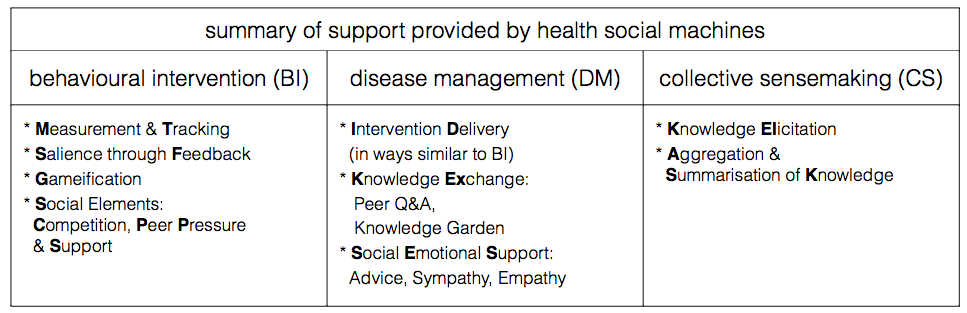
\includegraphics[width=13cm]{img/table2-summary.png}
\caption{\emph{Support offered by type of machine} - Summary of all of
  the types of support identified across machines, described in
  Section \ref{sec:support}, organised by type of machine.} \label{fig:summaryofsupport}
\end{center}
\end{figure*}


In order to understand better how the social machines just described
functioned to help individuals with their health related goals, we
performed an analysis of each site/app's features and derived a set of
observations pertaining to how they supported the goals each sought to
achieve.  We describe each, in turn, next

\subsection{Supporting behaviour change}
\label{sec:intervention}

In order to support individuals to conform to their behaviour change
interventions, we identified the following elements that these machines
support.

\begin{enumerate}
\item \emph{Measurement and Tracking} - As described earlier, in order
  to be able to provide feedback on progress, most of the machines
  provided support for some degree of data collection, ranging from
  facilitating manual data recording to automatically sensing activity
  and physiological signals through wearable sensors.
\item \emph{Salience and Feedback} - To remind individuals to comply
  with their intervention and reinforce encouragement for incremental
  progress, individuals' progress was made highly salient using a
  number of mechanisms.  For wearable sensors, visible indicators
  (lights/displays) on the sensor often indicated progress, while for
  apps and services, visual prompts, messages and alerts delivered
  through social networks, e-mail, text messages, and asynchronous
  ``push'' notifications were common.
\item \emph{Gamification (Achievements and Prizes)} - To futher
  motivate compliance, many of these systems incorporated a number of
  ``gamification'' features \cite{Deterding:2011:GUG:1979742.1979575}
  meant to make progres seem like play.  Such features typically
  involved rewarding participants with ``points'', ``badges'' and
  ``prizes'' for achieving milestones.
\item \emph{Social encouragement} - In addition to the individual
  gamification elements, social features were provided for most
  machines that encouraged indivdiuals to either compete to achieve
  their objectives either individually or in groups, or to support one
  another by ``cheering them on'' and supporting them in various ways.
  Competitive elements included ``battles'' and ``challenges'', supportive
  capabilities included ``cheerleading'', wagering, and donating ``points''
  in support of another individual's cause.
\end{enumerate}

\subsection{Facilitating disease management}
Disease management machines provide three kinds of support to
individuals; first, like the behavioural intervention machines, to
deliver actual interventions specific to individuals' conditions.  One
of the best examples of such intervention delivery is BigWhiteWall\footnote{The Big White Wall - \url{www.bigwhitewall.com}},
which delivers mental health services through an online social network
through a full-time staff of professional counselors who monitor the
site 24 hours a day.

The second role these marhines serve is a place to exchange knowledge
and insight, serving as both \emph{answer gardens} \cite{answergarden}
and \emph{serendipitous knowledge archives} \cite{knowledgearchive}.
As answer gardens, these sites let individuals find and post answers
to specific questions they have.  As knowledge archives, individuals
with similar circumstances can post and more easily stumble upon tips
that are relevant to their particular situation(s) - which might help
them improve their situation (even if they did not know to
specifically ask or look for this information to begin with).

Third, these systems provide a mechanism of social emotional support,
both in terms of empathy from people who have experienced similar
situations in the past, or sympathy, from those who can relate and
provide words of encouragement or advice.

\subsection{Enabling crowd-based sensemaking}

Health machines that seek to crowdsource information about disease and
treatments at large scale require the ability to acquire information
effectively and as accurately as possible from participants.  Thus,
effective elicitation of information becomes a primary challenge.
Towards this capabillity, PatientsLikeMe supported a structured
elicitation approach for the gathering of symptoms, relevant diagnosed
diseases, treatments, and reports of experiences.  Gathering
structured data directly (in terms of ratings, diseases and treatments
from a fixed lexicon) allowed these data can be compared and
aggregated automatically across individuals.  

Beyond elicitation, such sites require the ability to produce useful
views of collected data so that participnats are not overwhelmed by
the volumes of raw data produced by others.  Towards this end,
PatientsLikeMe used the structured data captured to synthesize raw
simple aggregate visualisations and result summaries that could be
easily interpreted.

\section{Challenges and Limitations}
\label{sec:limitations}

In this section we synthesise a set of problems and challenges that
have been voiced concerning the effectiveness of health social
machines, including concerns voiced by the medical community. 

\subsection{Potential Dangers of Self-Diagnosis}

Many of the examined machines encourage individuals to make their own
decisions concerning their health, with such slogans as ``take back
your health now!''.  To do this, they give seemingly appropriate and
relevant information to individuals that let them choose options, such
as intervention programmes, or, in the case of PatientsLikeMe,
treatments from which to choose.  One of the appeals of this idea is
that if individuals are the ones that choose their intervention, they
would feel more ownership over it and would be more likely to comply
fully.

However, clinicians and medical professionals have voiced concern
about this intiiatve, because individuals lacking medical expertise or
experience are likely to make bad decisions on incomplete knowledge
that may put their health in peril.  For example, an individual who is
feeling unwell might suspect that they need more physical exercise and
sign up to an ``increased activity'' intervention programme, when in
fact they might have a heart condition that might become more severe
under increased cardiovascular strain.  If they had seen a medical
professional instead of self-diagnosing themselves, the heart
condition may have been identified earlier and more easily addressed.

\subsection{Quality and Adherence to Intervention Programmes}

A second associated concern pertaining to democratising the creation
and administration of intervention programmes is simply, first, that
having non-medical professionals devise intervention programmes means
these programmes have not been rigorously evaluated, and thus may be
less effective (or entirely ineffective) beyond a placebo effect
\cite{placeboeffect}.  

Furthermore, professional clinicians, therapists and psychiatrists
have methods to make sure individuals are comply and adhere with their
intervention and receiving maximum benefit.  When the professional is
removed from the loop, interventions may become less effective as
patients are not guided to adhere to the prescribed programmes. Thus
other mechanisms (such as the gamification components described above)
will need to fill this role.

On the other hand, the potential for the new wearbale sensor activity
monitors means that an indivdiual's activities can be recorded at
little or no cost, and analysed to produce a more complete picture of
an individual's activities; this could be useful in increasing
compliance and understanding of how an individual is behaving and can
improve their performance.

\subsection{Sustaining Motivation}
\label{sec:motivation}
A second challenge concerns the effectiveness the methods applied by
health social machines towards sustaining long-term involvement, in
particular for encouraging compliance and adherence to the more
difficult intevenions that challenge the very centres of people's
motivational systems, such as those concerning weight loss and
mental health.

In particular, a number of recent studies on gamification have
revealed that simple approaches for introducing extrinsic reward, such
as points and ``badges'' may wear off after a short initial period of
novelty \cite{therebedragons}.  Even the most successful example of
gamification, Foursquare, experienced a widespread engagement problem
across its user population six to 12 months after adoption
\cite{browningattheedges}. Meanwhile, other studies of gamification
showed that gamification elements actually decreased participation by
reducing individuals' intrinsic motivation to participate, which, in
some cases returned when the gameificaiton elements were once again
removed \cite{Thom:2012:RGE:2145204.2145362}.

\subsection{Self-Report, Bias and Explaining-Away}

In the realm of crowd-sourcing disease knowledge, several of the
health machines rely on self-report as the primary method of knowledge
elicitation.  Controlled studies have demonstrated the many problems
of self-report across domains, with the most significant biases being
revealed in health, such as concerning a person's estimates of their
own fitness, including body mass and weight \cite{elgar2005validity}
and happiness, including depression \cite{hunt2003self}. Such biases,
which vary among individuals and factors estimated, could
significantly impact the validity of the data collected if it is
information concerning the diseases and symptoms.

Of additional difficulty concerning self-report arises in situations
where there is need for patients to perform causal inference between
symptoms, causes and treatments, such the case with PatientsLikeMe,
which asks patients to describe symptoms experienced with a disease
and the outcome of particular treatments.  The well-studied
psychological effect of confirmation bias \cite{confirmationbias},
which causes individuals to gather evidence in support of pre-existing
beliefs, could cause individuals to report what they \emph{think they
  should see} instead of what they actually experienced.  Furthermore,
illusory correlation \cite{chapman1969illusory} could cause
individuals to draw connections between experiences, situations or
conditions merely due to their salience or co-occurrence, rather than
due to an actual causal relationship. A particular type of illusory
correlation is \emph{explaining away}, in which individuals attribute
causes to the most salient explanation, rather than the most probable
one \cite{gilovich1983biased}.

An additional bias that emerges when self-reports are produced in
groups is \emph{collective conservatism}, a very strong bias that
people in a group tend to say (or agree with) what others say instead
of contributing what they actually observe, feel or know.  This
phenomenon, well studied in social psychology
(e.g. \cite{aronson2003readings}), has been shown to cause individuals
to conform to, and even believe, incorrect group conclusions even when
they disagree with these conclusions themselves.  In public discussion
forums such as PatientLikeMe, collective conformation could dramatically
shape the conclusions that patients arrive at, and that future patients
might experience.

\subsection{Device and App-centricity}

An additional problem pertains to the fact that a majority of the
current behavior intervention machines described earlier are highly
device and app-centric; that is, the sensor(s) and app(s) designed to
record data are closely integrated with the methods for storing the
data, and the intervention delivery mechanisms.  This means that, in
these machines, the device and app makers retain the data collected
about and by users, and specified the kinds of interventions that are
possible, often in a one-size-fits-all approach.  This
vendor-centricity precludes the kinds of highly personalised,
multifaceted medicine which is likely to be more effective in the long
term, which may, for example, require use of several different
activity recording devices and interventions in tandem.

\section{Towards Better Health Machines}

In this section, we discuss ways to address the limitations described
in Section \ref{sec:limitations}, towards making health social
machines more versatile, robust and effective in the long term.

\subsection{Educating patients while empowering, not replacing, medical professionals}

While goals of greater patient-empowerment are likely to allow
individuals to make better health-related decisions in the long term,
the idea of health social machines should \emph{replace} the expert
assessments of trained medical profesionals seems ill-advised for the
foreseeable future. Instead, we proppose to think of health social
machines as mechanisms for giving individuals both a greater literacy
about their health concerns and conisderations, and a mechanism by
which individuals can effectively eliminate barriers to the best
medical experts and expertise available, whenever and by whomever it
is needed.

If medical consultations with professionals were shared in a
PatientsLikeMe social machine context, a number of benefits could be
gained.  First, patients could weigh and assess several options about
difficult medical decisions, using advice from others who have had to
make similar decisions in the past.  Furthermore, if such opinions
were shared in such forums, there will be pressure on clinicians to
provide their best, carefully assessed medical opinion for
individuals, since such opinions might be scrutinised by their peers
and the general public.  Such transparency would make visible the
track records of such professionals, and essentially give
professionals ``public reputations'' that could further be used by
individuals to make decisions about whom they should trust and why.

In such a scenario, medical specialists would see increasing demand
for their attention from individuals throughout the world for their
opinion, and would likely benefit from being able to increase the
efficiency and effectiveness with which they can assess the
condition(s) of the patients they see.  Here, additional health social
machine technology could come into play; specifically, the monitoring
sensors used in the behavioural intervention machines discussed in
Section \ref{sec:intervention} could be instead appropriated as
general-purpose health monitors which could give specialists
unprecedented, accurate access to an individual's daily activities and
health.  This information could give doctors valuable context for
understanding each patient's lifestyle between visits, in order to
devise more appropriate interventions.

%% A number of challenges pertain to giving practitioners and
%% professionals then, suitable tools to let them cope with the demand of
%% potentially millions of individuals that would like their opinion. One
%% tool that might enable them to gain a quick and effective
%% understanding of a patient's condition would be

\subsection{Motivation and commitment}

As mentioned in Section \ref{sec:motivation}, the gamification
approaches currently used to motivate individuals to comply with
behaviour change intervensions are likely to prove insufficient for
longer-term, more difficult programmes. Since compliance is mandatory
for succesfully applying interventions, this is an area where
formidable challenges remain.

Behavioural economics may provide insight towards approaches that
might work.  For example, Thaler and Susstein, authors of \emph{Nudge}
\cite{nudge}, cite several examples of using individuals' \emph{loss
  aversion} techniques to dramatically motivate individuals who have
important goals they need to keep.  Specifically, they provide two
examples where individuals committed to paying their friends or
academic advisors large sums of money if they failed to meet
particular goals each month (such as turning in a chapter of a
dissertation or losing a specified number of pounds).

Due to the importance of motivation, it may make sense to use a
combination of approaches.  For example, traditional fitness clubs and
``gym memberships'' provide a combination of pressures to keep members
attending and participating; first, they cost substantial membership
fees, which, at least for budget-conscious participants provide an
incentive to participate; second, they provide a number of strong
social pressures and expectations -- both from instructors and peers,
in which missing sessions could cause considerable embarassment.

\subsection{Making better use of sensed data }

Finally, we believe that decoupling sensing of individuals' physical
activities and vital statistics from device manufacturers' apps that
prescribe fixed functionality for such data will simply allow
individuals to make better use of their activity records.  In
particular, liberating this data for use by general application
developers will help inspire innovation in new sensor-enabled fitness
apps, without necessitating such vendors to flood the market with
their variation of nearly-identical sensing devices -- a phenomenon we
are witnessing today.

Giving individuals access to this valuable data, and ability to store
it longitudinally over time should motivate people to continue to log
and record important aspects of their physical activity and vital
statistics, so they can better understand their lifestyle and ways that
their behaviour impacts their general wellbeing.

\section{Conclusion}

The level of interest and engagement with the first generation of
health social machines suggests that people are eager to try and
evaluate new, social technologies that can potentially help them
improve their health and well-being. In this paper, we have
contributed a analysis of ways that this current generation of social
machines have been designed to play today, and the primary kinds of
challenges that these health support and intervention roles face
towards being made more effective, paritcularly in their delivery of
longer-term interventions We have proposed several new ideas towards
overcoming the most significant of these, including providing
facilities by which social machines can start to deliver on all three
of the key facilities -- behavioural intervention, disease management
and mitigation, and collective sensemaking in a more integrated way,
and ways by which medical professionals can use the machines to 
improve the way they interact with patients at scale, rather than
being excluded from the process.

%% individuals play in the machine, the
%% kinds of support received and given, and the overall objectives
%% sought.  We then described a number of challenges towards making these
%% machines achieve their ultimate goals, pertaining to the methods used
%% to motivate participation, elicit knowledge, and the general notion of
%%patient-centered diagnosis. 

%% 
%% Gym Membership: Thaler & Susstein
%% Group bias :: it's all in the knowledge elicitation
%%

% \section{Approaches}
%% \subsection{Social pressure and Motivation: Gym Memberships and Personal Trainers}
%% \subsection{Present: Channel factors, access, convenience}
%% \subsection{Present: Salience and reminders}
%% \subsection{Futures: Personalised Activity Diaries}
%% \subsection{Futures: Citizen-medicine}

\section{Acknowledgments}

This work is supported under SOCIAM: The Theory and Practice of Social
Machines.  The SOCIAM Project is funded by the UK Engineering and
Physical Sciences Research Council (EPSRC) under grant number
EP/J017728/1 and comprises the Universities of Southampton, Oxford and
Edinburgh.

%
% The following two commands are all you need in the
% initial runs of your .tex file to
% produce the bibliography for the citations in your paper.
\bibliographystyle{abbrv}
\bibliography{health-social-machines}  % sigproc.bib is the name of the Bibliography in this case
% You must have a proper ".bib" file
%  and remember to run:
% latex bibtex latex latex
% to resolve all references
%
% ACM needs 'a single self-contained file'!
%
%APPENDICES are optional


\balancecolumns % GM June 2007
% That's all folks!
\end{document}
